\chapter{Conclusións}
\minitoc
\label{chap:conclusiones}
\vspace{0.5cm}

%%%%%%%%%%%%%%%%%%%%%%%%%%%%%%%%%%%%%%%%%%%%%%%%%%%%%%%%%%%%%%%%%%%%%%%%%%%%%%%%
% Objetivo: Contar cómo está ahora el proyecto, si ha merecido la              %
%           pena, lo que se ha aprendido, si se aplicaría de nuevo, etc.       %
%%%%%%%%%%%%%%%%%%%%%%%%%%%%%%%%%%%%%%%%%%%%%%%%%%%%%%%%%%%%%%%%%%%%%%%%%%%%%%%%

\lettrine{N}{este} capítulo exporanse as conclusións do proxecto: desde as
múltiples incidencias, as maneiras de resolvelas e as leccións que se
aprenderon delas, ata as oportunidades de mellora ou futuras liñas de traballo.

\section{Incidencias durante o desenvolvemento do proxecto}

 \subsection{Planificación}

  \subsubsection{Xestión do proxecto}

  Como se comentou no capítulo \ref{chap:planificacion}, nun primeiro momento
  escolleuse \textit{OpenProj} coma xestor de proxectos, procedendo a meter
  nel toda a planificación. Todo ía ben, ata que un día fallou sen explicación
  aparente. \\

  Por motivos de dispoñibilidade de tempo do proxectando (estudos, traballo,
  etc.) decidiuse empregar un calendario de media xornada para o proxecto. Pois
  resulta que \textit{OpenProj}, alomenos na súa última versión liberada
  (v1.4-2, do 02/10/2008), presenta problemas á hora de manexar calendarios que
  non son o calendario por defecto (xornada completa). \\

  Concretamente, o erro deuse un día calquera ó abrir o ficheiro do proxecto
  cando, sen explicación aparante e sen ter cambiado nada, pasou de empregar un
  calendario de media xornada a un de xornada completa composto por dous de
  media xornada. É dicir, o que fixo foi meter nun mesmo día dúas medias
  xornadas e, polo tanto, reducir o intervalo estimado de datas á metade. A
  partires dese momento, aínda sen ter salvado os cambios, o erro reproducíase
  sempre. \\

  Dito problema non é salvable polo usuario de ningunha maneira sen
  distorsionar os datos da planificación, polo que é preciso corrixilo no
  código da aplicación. Investigando pola rede, parece ser que o erro estaba xa
  corrixido na seguinte versión, pero dita versión non era libre e non tiña
  visos de chegar a selo en moito tempo (\textit{OpenProj} tamén cunha versión
  comercial). \\

  Por dito motivo, tocou tirar coa planificación feita e volver comezar. Do que
  quedaba na lista e guiándose polas recomendacións, seleccionouse
  \textit{Planner}. \\

  \textit{Planner} é un xestor bastante sinxelo e rápido. Perdíase algo de
  funcionalidade fronte a \textit{OpenProj}, pero dado o atraso acumulado e que
  as pequenas carencias que se lle vían eran mitigables, optouse por el
  igualmente. \\

  Houbo que refacer toda a planificación de cero, dado que os formatos non eran
  compatibles e a xestión da información é totalmente diferente. \\

  Todo perfecto, ata que tocou asignar recursos materiais ás tarefas.
  Seleccionada a primeira tarefa, que xa tiña asignado un recurso humano,
  asígnaselle un recurso material e de repente a duración da tarefa redúcese á
  metade. É dicir, os recursos materiais consomen esforzo. En resumo, que os
  recursos materiais traballan. Para entenderse, se nunha tarefa se emprega,
  por exemplo, un paquete de folios, ese paquete traballa. Inadmisible. \\

  Isto pode ter sentido para recursos máquina, onde pode ser necesario
  contabilizar as horas de traballo da maquinaria, pero non para recursos
  materiais en xeral e sen posibilidade de decisión ó respecto.\\

  Notificáronse este e outros erros ós desenvolvedores, que procederon a
  marcalos todos coma duplicados, cando moitos deles non o eran e o resto tiñan
  un título moito máis descriptivo que os que xa había (polo que non se
  atoparon nunha busca previa). Ademais, agrupáronos todos nun único erro
  ``caixón de xastre'' sen relación. Por este último motivo e logo de que máis
  profesionais lles insistiran e non obtiveramos resposta algunha, desbotouse
  tamén o \textit{Planner}.\\

  Na lista restaban por probar \textit{GanttProject} e \textit{LibrePlan}.
  Analizando un pouco máis en profundidade o \textit{GanttProject} chegouse á
  conclusión de que era demasiado sinxelo (por non dicir incompleto) polo que
  se desbotou sen máis.\\

  Chegados a este punto, só quedaba \textit{LibrePlan}: servidor web, base de
  datos, interface web, multitude de opcións a priori complexas, xestión de
  información totalmente distinta a todo o visto anteriormente, alta curva de
  aprendizaxe e un longo etcétera.\\

  Volta outra vez a facer a planificación de cero. Ardua tarefa dada a
  lentitude da interface web. Tamén se detectou algún erro leve (corrixido en
  versións posteriores) e outro que parecía grave e ó final non era máis que o
  descoñecemento moi especifico que \textit{LibrePlan} marca por defecto e que
  se atopa bastante agochado. \\

  Con \textit{LibrePlan} deuse tamén unha incidencia grave, froito dun erro do
  entorno de escritorio do sistema operativo empregado. Nunha das múltiples
  actualizacións da aplicación, non se reconfigurou a base de datos por quedar
  oculta a fiestra de xestión da configuración, o que ocasionou que a
  aplicación se actualizase pero a base de datos non, facendo romper a primeira
  e corrompendo a segunda. \\

  Gracias ó traballo da xente detrás de \textit{LibrePlan} puido recuperarse a
  base de datos e con ela a planificación no mesmo estado que antes de
  corromperse.

 \subsection{Deseño do sistema}

  \subsubsection{Prototipo 3}

   \paragraph{Prototipo hardware}\mbox{}\\

    \subparagraph{Receptor XBee}\mbox{}\\

    Como se comentou no capítulo \ref{chap:diseno}, empregar un
    \textit{XBee Explorer USB} \cite{XBeeExplorer} (figura
    \ref{figura:XBeeExplorer}) como base do receptor XBee plantexaba un
    problema.

    \begin{figure}[htbp]
     \centering
     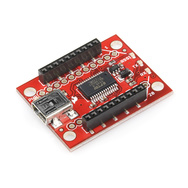
\includegraphics[scale=3.0,keepaspectratio=true]{./imagenes/xbee-explorer.jpg}
     % xbee-explorer.jpg: 188x188 pixel, 300dpi, 1.59x1.59 cm, bb=0 0 45 45
     \caption{XBee Explorer USB}
     \label{figura:XBeeExplorer2}
    \end{figure}

    Empregando esta placa, o dispositivo sería recoñecido no equipo coma un
    dispositivo USB, non coma un dispositivo MIDI, que é o que precisamos en
    última instancia. Por este motivo, habería que crear un controlador
    software para este dispostivo que fixese a conversión de USB a MIDI, para
    que puidese ser recoñecido polo sintentizador. Isto implicaría un retardo
    considerable (que seguramente dese ó traste co requisito de tempo real) e
    ademais, implicaría desenvolver un controlador distinto por cada familia de
    sistemas operativos. Como se pode intuir a simple vista, esta opción non
    era viable. \\

    Así que houbo que investigar un pouco para ver se había maneira de facer
    dita conversión por hardware, de tal maneira que ó enchufar o receptor vía
    USB fose recoñecido coma dispositivo MIDI, aforrando unha capa intermedia,
    un retardo importante e un esforzo máis ca considerable. \\

    Mirando o esquema do \textit{XBee Explorer USB} pódese ver que leva un chip
    \textit{FT232RL} (que é o que se encarga de facer a conversión de FTDI a
    USB) que, segundo pon aquí \cite{FT232RL} e aquí \cite{Moco}, non é posible
    reprogramar para facer unha conversión a MIDI. \\

    Segundo comentan tamén na segunda referencia, ese mesmo chip era o que se
    empregaba ata a versión \textit{Duemilanove} \cite{ArduinoDuemilanove} da
    placa estándar \textit{Arduino}, polo que tampouco era posible facelo con
    unha destas placas ata dita versión. \\

    A partires desa versión, cambiouse dito chip polos da familia
    \textit{Atmel Mega XuY} (8u2, 16u2, 32u4). Comezouse polo
    \textit{Arduino Uno} (8u2), que na súa terceira revisión o cambiou polo
    16u2 \cite{ArduinoUno}. E actualmente, a última placa que acaban de sacar,
    a \textit{Arduino Leonardo} \cite{ArduinoLeonardo} leva o 32u4. \\

    Dito chip está programado para funcionar exactamente igual que o
    \textit{FT232RL}, pero coa salvedade de que se pode reprogramar totalmente,
    polo que se pode empregar calquera placa \textit{Arduino} con dito chip
    para facer a conversión. \\

    Aínda que no momento de escribir estas liñas xa está dispoñible unha placa
    nova \cite{ArduinoLeonardo} que quizáis nos resultase máis sinxela de
    reprogramar, pois xa conta con USB nativo (sen necesidade de facer
    conversión serie-USB, polo que o novo firmware sería máis sinxelo), no
    momento de realizar o deseño hardware a última placa era a
    \textit{Arduino Uno r3}, que é un pouco máis completa, pero non conta con
    USB nativo. \\

    Sen embargo, se nos fixamos outra vez na referencia \cite{Moco}, vemos que
    xa a partires da revisión 2 (8u2) existe un firmware que fai este cometido,
    polo que se aforra moito tempo e esforzo. O esquema de funcionamento é o da
    figura \ref{figura:Moco2}.

    \begin{figure}[htbp]
     \centering
     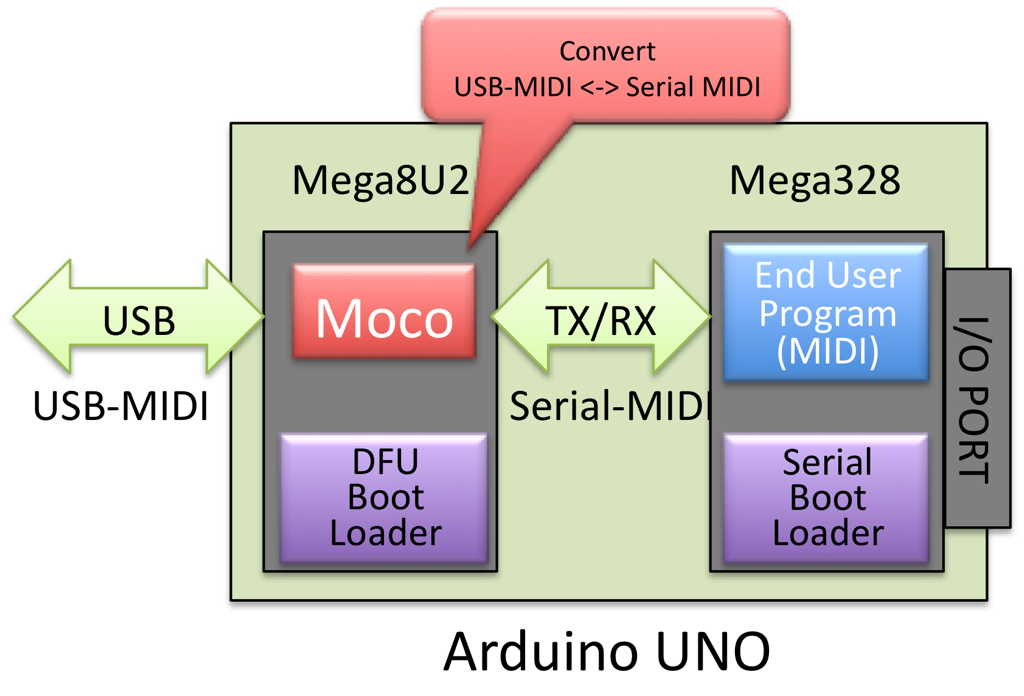
\includegraphics[scale=0.3,keepaspectratio=true]{./imagenes/moco.jpg}
     % moco.jpg: 1024x696 pixel, 72dpi, 36.12x24.55 cm, bb=0 0 1024 696
     \caption{Moco}
     \label{figura:Moco2}
    \end{figure}

    Ademais, polo que se pode ler ó final do artigo:

    \begin{quotation}
     \slshape
     Moco firmware can use as USB-MIDI \verb|<->| USB-Serial bridge with a 8u2
     or 32u4 board, like Adafruit’s 32u4 breakout board.
    \end{quotation}

    Vemos que dito firmware tamén funciona co chip 16u2 (que simplemente é un
    8u2 con máis memoria) e co 32u4 (que é o máis recente), polo que
    actualmente funciona con tódalas placas \textit{Arduino} lanzadas dende o
    \textit{Arduino Uno r2}. \\

    Polo que finalmente se optou por empregar como base do receptor un
    \textit{Arduino Uno} con firmware \textit{Moco}.

    \subparagraph{Fritzing}\mbox{}\\

    Como se comentou no capítulo \ref{chap:diseno}, a intalación de
    \textit{Fritzing} foi problemática. Instalada a versión dispoñible no
    repositorio da distribución en uso, comprobouse que a base de datos non
    contaba cunha gran cantidade de pezas. Procedeuse a comprobar a versión
    instalada (0.6.3) e cotexala coa última dispoñible nese momento (0.7.7b).
    Detectado o problema, intentouse compilar a versión dispoñible na web, pero
    non foi posible por mor de dependencias non localizables. A solución ó
    problema da escaseza de pezas da base de datos da versión do repositorio
    pasou por hackear a mesma, substituíndoa pola da versión máis recente (que
    contaba cun número de pezas moito máis elevado). \\

    Tamén se deron incidencias coas pezas a usar. A única reseñable por ter
    dado algo máis de traballo foi a que se deu co módulo de almacenamento, o
    \textit{MicroDrive G1}. \\

    Como se comentou no capítulo \ref{chap:diseno}, non estaba na base de datos
    do software por ser dun fabricante menos coñecido. Afortunadamente, estaba
    dispoñible no apartado de contribucións do repositorio da aplicación
    \cite{FioContribucionsFritzing}. Unha vez descargada, intentouse
    incorporala ó proxecto, pero non foi posible, pois tiña algún tipo de erro
    (e por iso non estaba incluida na base de datos). Investigando a fondo o
    ficheiro do proxecto (empregando un titorial \cite{TitorialFritzing} como
    guía), de formato \textit{fzp} (que non deixa de ser un XML) atopouse un
    erro na ruta ás diferentes vistas da peza (en formato svg), pois non
    coincidían totalmente os nomes dos ficheiros. Solventado o problema
    (hackeando o XML a man), procedeuse á súa incorporación ó proxecto. Así
    mesmo, notificouse o erro ós desenvolvedores da aplicación, contribuíndo a
    versión corrixida ó repositorio do proxecto \cite{ContribucionFritzing}.
    
 \subsection{Implementación}
 
  \subsubsection{Ensamblado e codificación}
  
   Durante a fase de ensamblado e codificación, unha vez tiñamos toda a
   codificación da parte hardware lista para probar, xurdiu un problema co que
   non contabamos en absoluto: a falta de memoria RAM da placa para executar o
   firmware programado. \\
   
   Todo ía ben e xa tiñamos codificado e compilando os tres módulos dos
   periféricos, e o software de integración de todos eles e que conforma o
   simulador do punteiro en si, pero cando fomos compilar todo o conxunto,
   previo á súa carga na placa Arduino Uno, o IDE díxonos que a compilación
   estaba ben, pero que o tamaño do executable excedía o máximo da memoria RAM
   nun 9\% e propúñanos intentar reducir o número de variables globais para
   intentar mitigalo (figura \ref{figura:ConsumoMemoria}). \\
   
   \begin{figure}[htbp]
    \centering
    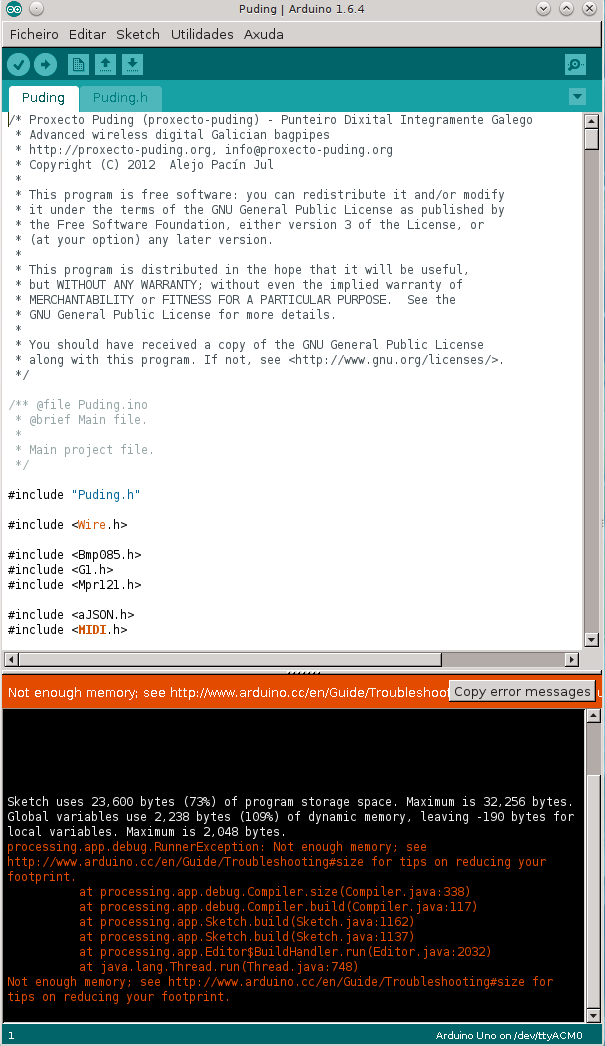
\includegraphics[scale=0.6,keepaspectratio=true]{./imagenes/consumo-memoria.png}
    % consumo-memoria.png: 1024x696 pixel, 72dpi, 36.12x24.55 cm, bb=0 0 1024 696
    \caption{Consumo de memoria}
    \label{figura:ConsumoMemoria}
   \end{figure}
   
   A primeira aproximación foi avaliar as variables globais da aplicación para
   ver o número delas, os seus tipos e se eran susceptibles de eliminación. \\
   
   E viuse que eran moi pouquiñas, que os tipos eran básicos e que non eran
   eliminables. Salvo un par de delas, que son concretamente as matrices
   constantes que conteñen as relacións predefinidas entre dixitación e
   desprazamento en semitonos desde a nota base. As coñecidas como dixitación
   aberta e pechada. \\
   
   O primeiro que nos chamou a atención foi que, sendo constantes, se
   almacenasen en RAM e non en ROM. Buscando a causa, a explicación é que a
   arquitectura empregada por Arduino, coas memorias separadas, fai que este
   tipo de variables constantes vaian parar á RAM. \\
   
   Vendo que non era posible que acabasen na memoria reservada a datos fixos,
   analizáronse os valores e vendo que nos chegaban 2 bytes para representalos,
   cambiáronse de tipo int a short, pero sorprendentemente a nivel compilación
   non se gañou nada. \\
   
   O último que probamos foi a movelas como variables locais á única función
   onde se empregaban, gañando temporalmente un 6\% de espacio de memoria, pero
   todavía insuficiente. \\
   
   Cómpre explicar que estas dúas matrices se empregan para cargar noutra matriz
   de dixitacións globais todas aquelas dixitacións que o usuario queira
   empregar, puidendo ser aberta, pechada ou personalizada a vontade, polo que
   hai que ter en conta que a memoria necesaria pode subir ata outro 10\% só
   tendo en conta esta matriz global. E aínda teriamos que deixar marxe para o
   resto de variables locais que, se facemos unha similitude con outros sistemas
   similares, podemos estimar nun 20\% extra. Polo que de maneira estimada e
   aproximada, estamos nun -36\% de memoria RAM dispoñible. \\
   
   Compilando o firmware coa última versión do IDE de Arduino instalada no
   equipo de implantación, conseguiu reducirse o consumo de memoria nun 3\%
   (senón por melloras do compilador, probablemente polo cambio de int a short
   que poida que si aplique ben nesta nova versión), pero seguía sendo
   insuficiente. No mellor dos casos, estamos falando dun -28\% de memoria
   dispoñible. \\
   
   Aclarar neste punto que, tanto a placa Arduino Uno como a Arduino Fio,
   contan exactamente coa mesma arquitectura e cantidade de memoria; no caso da
   RAM, 2K. \\
   
   Visto que non había maneira de salvar a restricción de memoria de maneira
   programática e avaliando as alternativas definidas ó inicio da iteración,
   decidiuse que a mellor opción era recortar módulos para alomenos ter algo
   funcional. \\
   
   Feitas contas e postos a escoller, a reproducción primaba sobre a
   configuración, polo que se prescindiu do lector de tarxetas, en detrimento
   tamén da aplicación de configuración. \\
   
   E posto que tampouco estaba claro como ía evolucionar o consumo de memoria
   das variables locais no tempo e que o IDE non proporciona dita información
   de ningunha maneira, por precaución, decidiuse prescindir tamén do sensor de
   presión e incorporalo posteriormente se había posibilidade. \\
   
   Polo que se prodeceu ó desenvolvemento dunha versión simplificada paralela
   que, unha vez rematada, arroxou un consumo de memoria mínimo do 72\% (figura
   \ref{figura:ConsumoMemoriaSimplficada}), que nos deixa exactamente no mínimo
   de RAM libre que teorizamos que nos faría falta para as variables globais
   non inicializadas previamente e as variables locais. \\
   
   \begin{figure}[htbp]
    \centering
    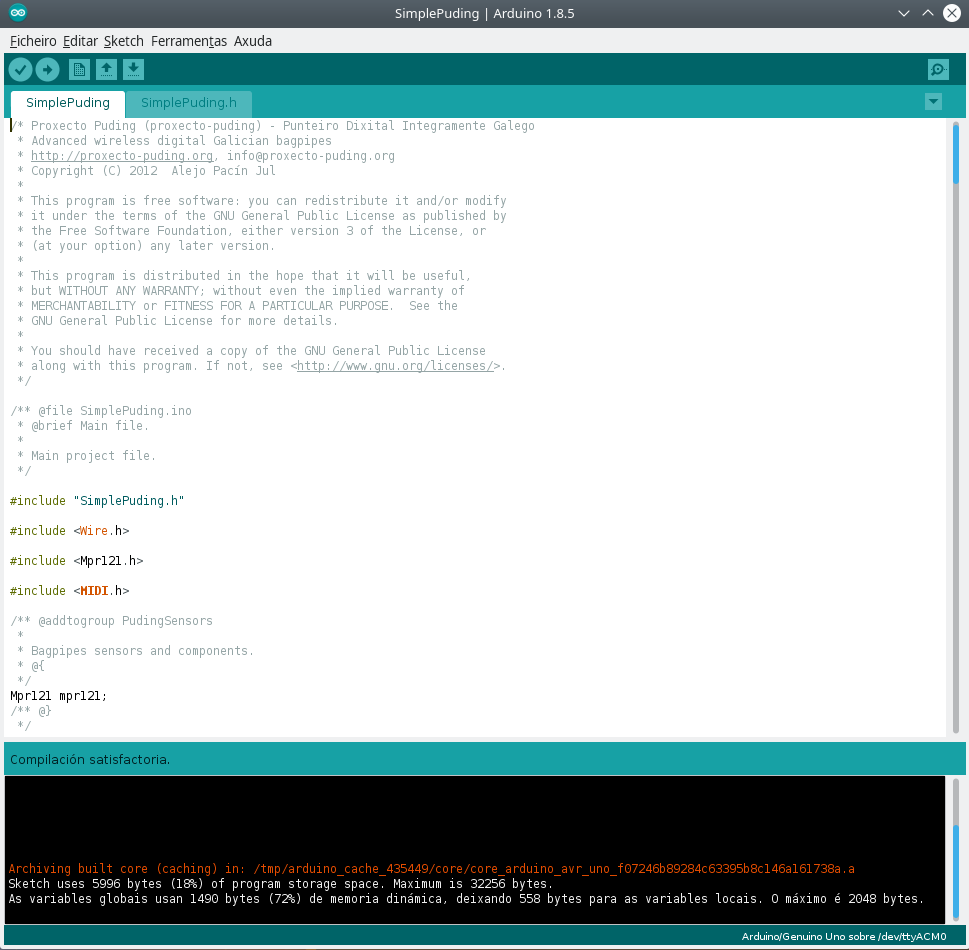
\includegraphics[scale=0.55,keepaspectratio=true]{./imagenes/consumo-memoria-simplificada.png}
    % consumo-memoria-simplificada.png: 1024x696 pixel, 72dpi, 36.12x24.55 cm, bb=0 0 1024 696
    \caption{Consumo de memoria da versión simplificada}
    \label{figura:ConsumoMemoriaSimplificada}
   \end{figure}
   
  \subsubsection{Integración e probas}
  
  Foito do problema comentado no punto inmediantamente anterior, dado que se
  anularon o sensor de presión e o lector de tarxetas, non foi posible probar
  e integrar a aplicación de configuración co dispositivo hardware, porque a fin
  de contas, non había hardware contra o que probar dita funcionalidade. \\
  
  Para mitigalo, tal e como se comentou durante a fase de probas, o que se fixo
  foi crear un simulador software o máis fiel posible ó dispositivo hardware a
  nivel de comportamento, de maneira que pudieramos validar tanto o fluxo de
  datos coma o seu formato.
  
  \subsubsection{Implantación}
  
  Por se os continuos problemas cos que nos atopamos durante o desenvolvemento
  do proxecto non fosen suficientes, a día 16 de agosto de 2018 o equipo co que
  se estaba a desenvolver o proxecto derramouse sen previo aviso, dificultando
  moito a finaliación do mesmo, pois estamos a falar de tres semanas vista ó
  límite de depósito da memoria, sen tempo case para maniobrar. \\
  
  Intentando tomar vantaxe do problema e logo de mercar un equipo novo de
  urxencia e preparalo para o seu uso, decidiuse empregalo tamén como banco de
  probas para unha implantación limpa. \\
  
  Durante todo o desenvolvemento do proxecto, logo dos múltiples problemas
  ocasionados por pequenas actualizacións do entorno de traballo, decidiuse
  mantelo estable durante a execución do mesmo, facendo que en última instancia
  contaramos cun sistema operativo, unha máquina virtual de Java e uns entornos
  de desenvolvemento totalmente desfasados, pero estables. \\
  
  De aí que, ó facer unha nova implantación de cero e aproveitando para probar
  coas últimas versións de todo o anterior, moitas das cales ían xa por varias
  versións maiores posteriores, se presentasen problemas novos. \\
  
  O proxecto foi incialmente pensado para OpenJDK 6 e posteriormente actualizado
  a OpenJDK 8 para aproveitar as novas funcionalidades de Java en aras de
  simplificar o desenvolvemento, pero a versión actual da instalada no equipo é
  a 11. \\
  
  A priori non deu problemas, ata que probamos a executar os tests do servizo de
  navegación web, que non funcionaban. Buscando a causa pola rede, semella que
  OpenJDK en versións posteriores á 8, rompeu varios enlaces simbólicos e outras
  partes relacionadas que afectan á carga das librerías de accesibilidade e que
  fai que a librería nativa do JDK que se emprega habitualmente para interactuar
  co escritorio independentemente do sistema operativo rompa en sistemas UNIX,
  polo que non permitía abrir o navegador web. \\
  
  Como solución de emerxencia mentres non arranxan a incidencia, que xa está
  notificada, engadiuse unha implementación alternativa en caso de erro facendo
  uso dunha librería equivalente da Apache Foundation.

\section{Conclusións finais}

 Lorem ipsum...
